\begin{exercise}
  Ziel dieser Aufgabe sit die Konstruktion eines Differenzenverfahrens für krumme
  Ränder. Sie dazu $E =(x_ic y_j) \in \R^2 \in \Omega$ ein Gitterpunkt im Inneren
  von $\Omega$, sodass die Gitterpunkte links $(x_i -h, y_j)$ und unterhalb
  $(x_i,y_j -h)$ von $E$ im Gebiet $\Omega$ liegen aber die Gitterpunkte rechts
  $(x_i + h, y_j)$ und oberhalb $(x_i, y_j + h)$ von $E$ nicht mehr in $\Omega$ liegen.
  Konstruieren Sie analog zu Aufgabe $59$ einen $5$-Punkt Differenzenstern für
  $\delta u(E)$, welcher $E$, die in $\Omega$ liegenden Nachbarpunkte $(x_i -h, y_j)$
  und $(x_i, y_j -h)$ sowie die Randpunkte
  $(x_i + \delta_x h , y_j), (x_i, y_j + \delta_y h) \in \partial \Omega$ mit
  $\delta_x, \delta_y \in (0,1)$ verwendet (siehe Abb. $2$). Welche Ordnung kann man
  erreichen?

  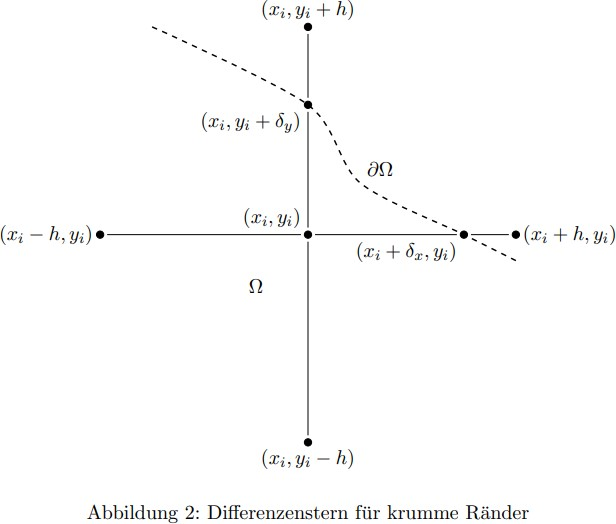
\includegraphics{Abbildung_2}
\end{exercise}

\begin{solution}
  Beweis.
\end{solution}
